\documentclass[10pt]{report}
\usepackage{fullpage}
\usepackage{graphicx}
\usepackage{verbatim}
\usepackage{subfig}

\newcommand{\HRule}{\rule{\linewidth}{0.5mm}}

\begin{document}
\begin{titlepage}
\begin{center}
% Upper part of the page

\includegraphics[width=0.15\textwidth]{logo.jpg}\\[2cm]    
\textsc{\LARGE CS 680}\\[1.5cm]

\textsc{\Large Computer Graphics}\\[0.5cm]


% Title
\HRule \\[0.4cm]
{ \huge \bfseries Air Hockey User and Technical Manual}\\[0.4cm]

\HRule \\[1.5cm]

% Author and supervisor
\begin{minipage}{0.4\textwidth}
\begin{center} \large
\emph{Author:}\\
Joshua \textsc{Gleason}
Marvin \textsc{Smith}
\end{center}
\end{minipage}
\vfill
% Bottom of the page
{\large \today}
\end{center}
\end{titlepage}
\newpage

%**************************************************%
%                    INTRODUCTION                  %
%**************************************************%
\section*{Air Hockey Overview}


\section*{Opinions}


\section*{Time Spent}



\section*{Extra Credit}
\begin{description}
\item[High Scores Window] accessible from either the menu or by pressing '8' key
\end{description}

%**************************************************%
%                    USER MANUAL                   %
%**************************************************%
\clearpage
\section*{User Manual}
\subsection*{Introduction}
This manual will introduce you to the basic functions of the AirHockey 
game. Figure \ref{fig:game} shows the basic layout of the game.

\begin{figure}[!h]
\centering
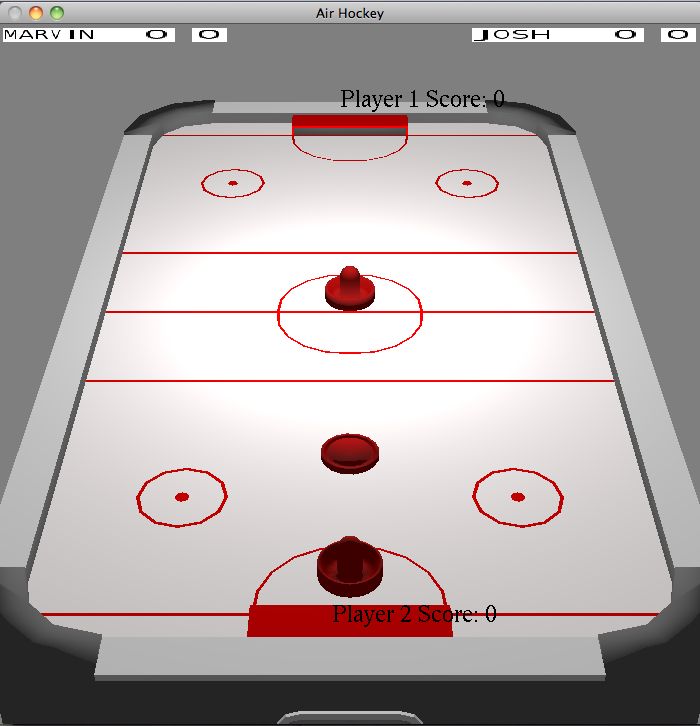
\includegraphics[width=3in]{game.png}
\caption{Basic Layout of Air Hockey}
\label{fig:game}
\end{figure}

Throughout gameplay, the user will have access to game state information through the
Heads Up Display (HUD). This is the bar at the top of the screen. The player names may be set
in the data/options.cfg file under the PLAYER\#\_NAME options. The first number to the right of the
names is the current score for that particular game. The second number is the number of player wins 
in the sequence. If the player wins enough games, the console will ask the user for their tag
at the end to add you in the Hall of Fame. This is described in more detail below. Figure 
\ref{fig:game} shows the HUD.

\clearpage
\subsection*{User Menu}
There are many different features in Air Hockey. To get to all of them, you will
need either the keyboard or the menu. To access the menu, click on the screen with
the right-mouse button. Figure \ref{fig:menu} shows the basic layout of the menu. 

\begin{figure}[!h]
\centering
\subfloat[Main Menu]{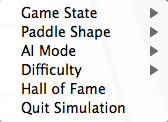
\includegraphics[width=1.3in]{menu.png}}
\subfloat[State Submenu]{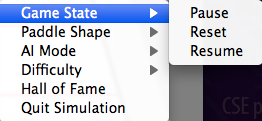
\includegraphics[width=1.8in]{menu_state.png}}
\subfloat[Shape Submenu]{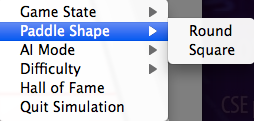
\includegraphics[width=1.7in]{menu_shape.png}}\\
\subfloat[AI Submenu]{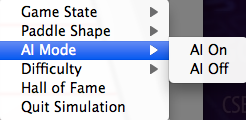
\includegraphics[width=1.6in]{menu_ai.png}}
\subfloat[Difficulty Submenu]{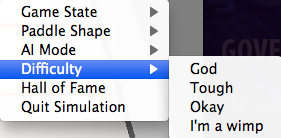
\includegraphics[width=1.7in]{menu_difficulty.png}}
\caption{Basic Menu Layout of Air Hockey}
\label{fig:menu}
\end{figure}

\noindent\underline{\textbf{Menu Options}}
\begin{description}
\item[Game State] Affects the gameplay action.
   \begin{description}
   \item[Pause Game] Halts game progress until resumed.
   \item[Reset Game] Clears the player score and starts the game over.
                     Will keep player wins however.
   \item[Resume Game] Will un-pause the game, allowing the game to step.
   \end{description}
\item[Paddle Shape] Affects the shape of the paddle.
   \begin{description}
   \item[Round] Round Paddle. See Figure \ref{fig:paddle}.
   \item[Square]Square Paddle. See FIgure \ref{fig:paddle}.
   \item \begin{figure}[!h]
         \centering
         \subfloat[Round Paddle]{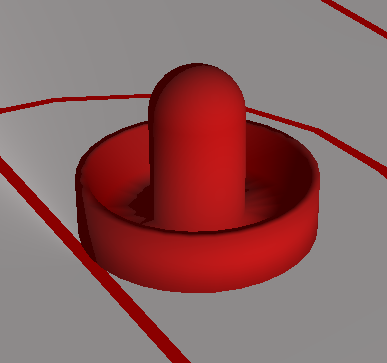
\includegraphics[height=2.5in]{round.png}}
         \subfloat[Square Paddle]{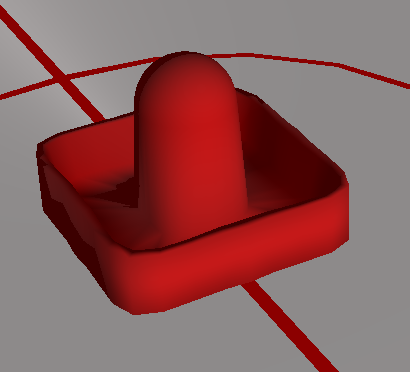
\includegraphics[height=2.5in]{square.png}}
         \caption{Paddle Shapes}
         \label{fig:paddle}
         \end{figure}
   \end{description}
\item[AI Mode] Toggles between single and double player modes.
\item[Difficulty] Determines the AI Skill Level
   \begin{description}
   \item[I'm a wimp] Don't bother, you already won. 
   \item[Okay] Default. The AI shows up to play.
   \item[Tough] You had better come ready for a fight. 
   \item[God]  If you can get the puck past the AI, you are better than me.
   \end{description}
\item[Hall of Fame] Show the top performers.
         \begin{figure}[!h]
         \centering
         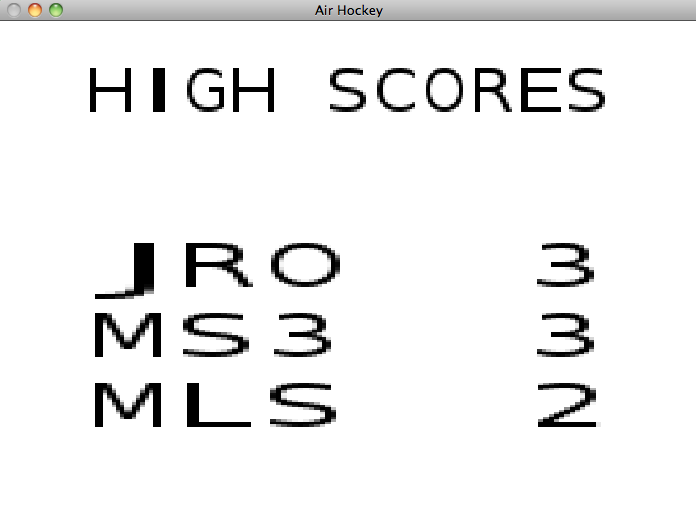
\includegraphics[height=3.0in]{hof.png}
         \caption{Hall of Fame Screen (Shows number of wins)}
         \label{fig:hof}
\item[Quit Simulation] Exit the program.
         \end{figure}
\end{description}

\clearpage
\subsection*{Keyboard Map}
\begin{table}[!h]
\centering
\begin{tabular}{|c|c|c|c|c|}\hline 
\textbf{Key}   & \textbf{Function}              &  &  \textbf{Key}   & \textbf{Function}  \\\hline
8              &  Show High Score               &  &  w  &  Move Camera Forward           \\\hline
               &                                &  &  s  &  Move Camera Backward          \\\hline
$\leftarrow$   &  Player 2 move paddle left     &  &  a  &  Shift Camera Left             \\\hline
$\rightarrow$  &  Player 2 move paddle right    &  &  d  &  Shift Camera Right            \\\hline
$\uparrow$     &  Player 2 move paddle up       &  &  q  &  Shift Camera Upwards          \\\hline
$\downarrow$   &  Player 2 move paddle down     &  &  e  &  Shift Camera Downwards        \\\hline
               &                                &  &  i  &  Rotate Camera Eye Upwards     \\\hline
m              &  Translate Light +Z axis       &  &  k  &  Rotate Camera Eye Downwards   \\\hline
n              &  Translate Light -Z axis       &  &  j  &  Rotate Camera Eye Left        \\\hline
.              &  Translate Light +X axis       &  &  l  &  Rotate Camera Eye Right       \\\hline
,              &  Translate Light -X axis       &  &     &                                \\\hline
               &                                &  &     &                                \\\hline
\end{tabular}
\caption{Keyboard Map of Air Hockey}
\label{tab:keyboard}
\end{table}

\subsection*{Camera}
The camera in our Air Hockey allows for complete motion and will enable the user to have any view of the
game that they wish. The camera controls are outlined in Figure \ref{tab:keyboard}. Figure \ref{fig:camera}
shows various views of the camera. 

\begin{figure}[!h]
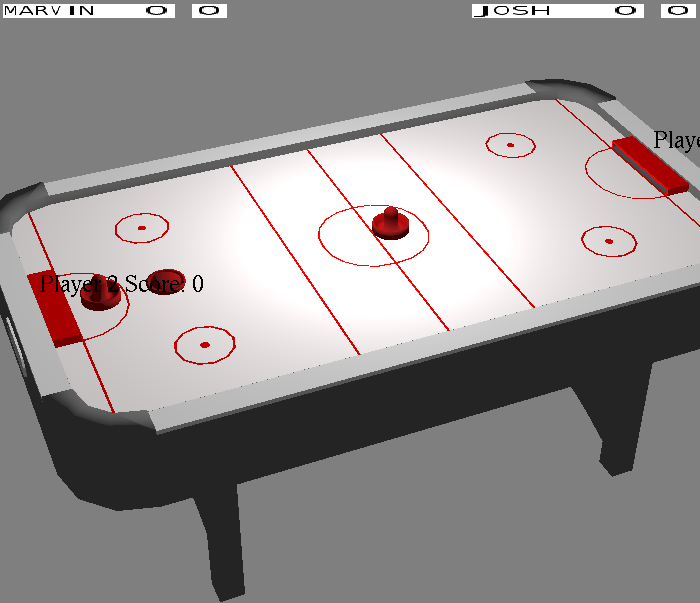
\includegraphics[width=2in]{camera1.png}
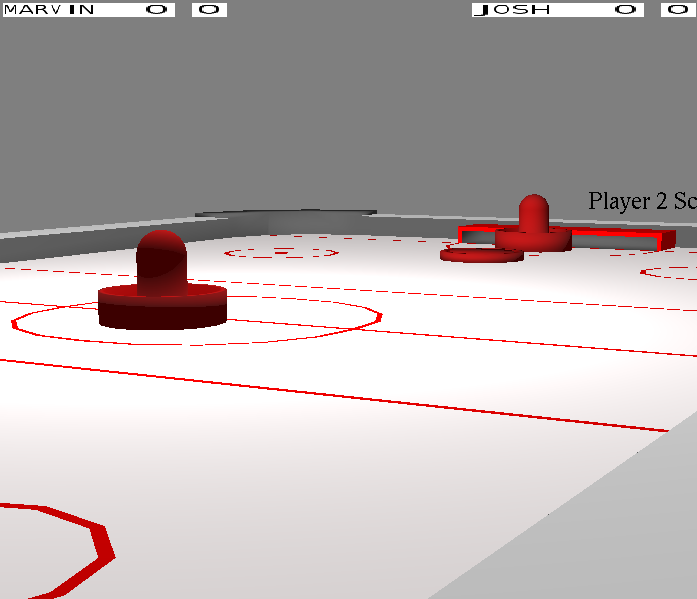
\includegraphics[width=2in]{camera2.png}
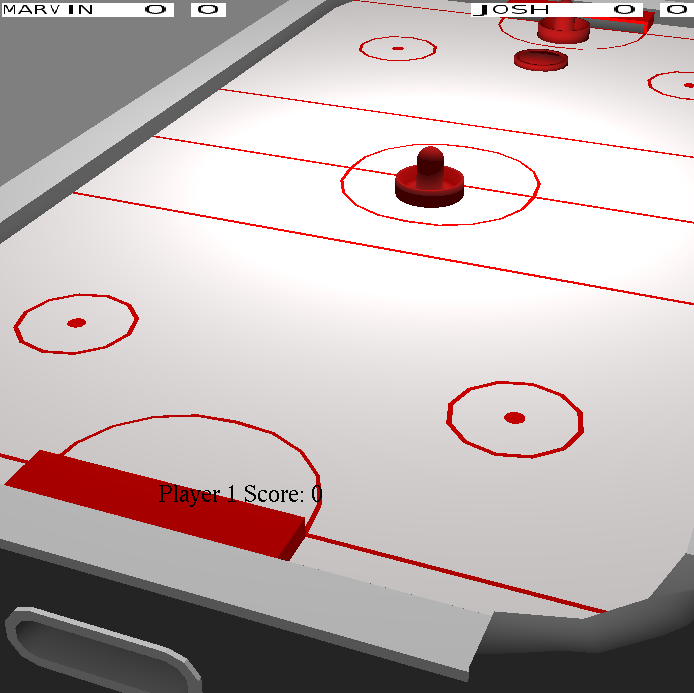
\includegraphics[width=2in]{camera3.png}
\caption{Camera Views Possible}
\label{fig:camera}
\end{figure}

\subsection*{Light Model}
The light model in Air Hockey allows for X and Z axis \emph{translation}. This will allow the user to see
effects of light and shadows. Figure \ref{fig:light} shows various light positions of the same scene.

\begin{figure}[!h]
\subfloat[Light Source Right of Camera]{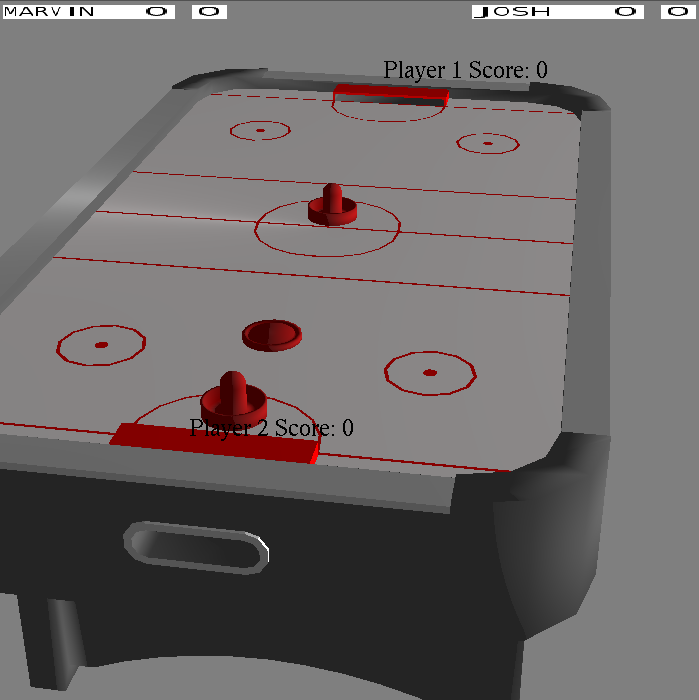
\includegraphics[width=2in]{light1.png}}
\subfloat[Light Source Behind Camera]{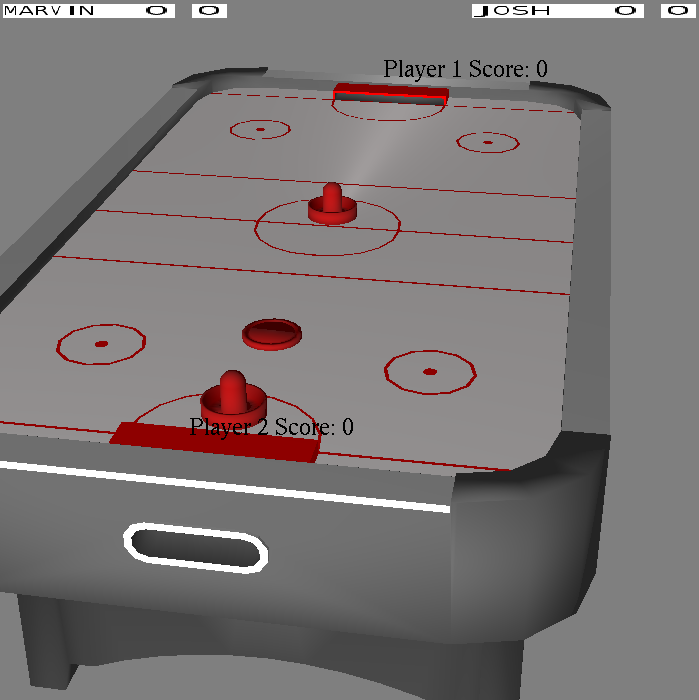
\includegraphics[width=2in]{light2.png}}
\subfloat[Light Source Away from Camera]{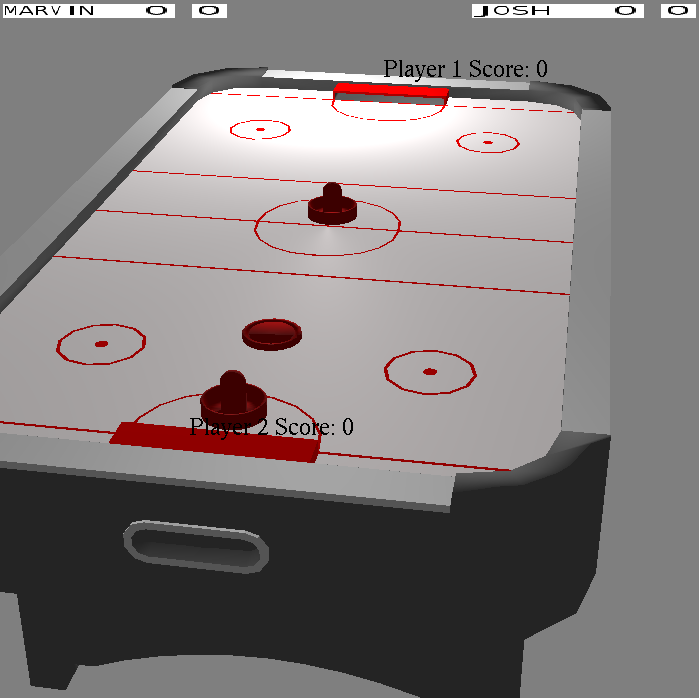
\includegraphics[width=2in]{light3.png}}
\caption{Light Model Examples}
\label{fig:light}
\end{figure}

\clearpage
\section*{Technical Manual}
\subsection*{Design Decisions}

\begin{description}
\item[something]
\end{description}

\subsection*{Deficiencies}

\subsection*{Areas for Improvement}

\end{document}
